% Options for packages loaded elsewhere
\PassOptionsToPackage{unicode}{hyperref}
\PassOptionsToPackage{hyphens}{url}
\PassOptionsToPackage{dvipsnames,svgnames,x11names}{xcolor}
%
\documentclass[
  letterpaper,
  twocolumn]{article}
\usepackage{amsmath,amssymb}
\usepackage{iftex}
\ifPDFTeX
  \usepackage[T1]{fontenc}
  \usepackage[utf8]{inputenc}
  \usepackage{textcomp} % provide euro and other symbols
\else % if luatex or xetex
  \usepackage{unicode-math} % this also loads fontspec
  \defaultfontfeatures{Scale=MatchLowercase}
  \defaultfontfeatures[\rmfamily]{Ligatures=TeX,Scale=1}
\fi
\usepackage{lmodern}
\ifPDFTeX\else
  % xetex/luatex font selection
    \setmainfont[]{Libertinus Serif}
    \setsansfont[]{Libertinus Sans}
    \setmonofont[]{Iosevka}
  \setmathfont[]{Libertinus Math}
\fi
% Use upquote if available, for straight quotes in verbatim environments
\IfFileExists{upquote.sty}{\usepackage{upquote}}{}
\IfFileExists{microtype.sty}{% use microtype if available
  \usepackage[]{microtype}
  \UseMicrotypeSet[protrusion]{basicmath} % disable protrusion for tt fonts
}{}
\makeatletter
\@ifundefined{KOMAClassName}{% if non-KOMA class
  \IfFileExists{parskip.sty}{%
    \usepackage{parskip}
  }{% else
    \setlength{\parindent}{0pt}
    \setlength{\parskip}{6pt plus 2pt minus 1pt}}
}{% if KOMA class
  \KOMAoptions{parskip=half}}
\makeatother
\usepackage{xcolor}
\usepackage[margin=1.3in]{geometry}
\usepackage{longtable,booktabs,array}
\usepackage{calc} % for calculating minipage widths
% Correct order of tables after \paragraph or \subparagraph
\usepackage{etoolbox}
\makeatletter
\patchcmd\longtable{\par}{\if@noskipsec\mbox{}\fi\par}{}{}
\makeatother
% Allow footnotes in longtable head/foot
\IfFileExists{footnotehyper.sty}{\usepackage{footnotehyper}}{\usepackage{footnote}}
\makesavenoteenv{longtable}
\usepackage{graphicx}
\makeatletter
\def\maxwidth{\ifdim\Gin@nat@width>\linewidth\linewidth\else\Gin@nat@width\fi}
\def\maxheight{\ifdim\Gin@nat@height>\textheight\textheight\else\Gin@nat@height\fi}
\makeatother
% Scale images if necessary, so that they will not overflow the page
% margins by default, and it is still possible to overwrite the defaults
% using explicit options in \includegraphics[width, height, ...]{}
\setkeys{Gin}{width=\maxwidth,height=\maxheight,keepaspectratio}
% Set default figure placement to htbp
\makeatletter
\def\fps@figure{htbp}
\makeatother
\setlength{\emergencystretch}{3em} % prevent overfull lines
\providecommand{\tightlist}{%
  \setlength{\itemsep}{0pt}\setlength{\parskip}{0pt}}
\setcounter{secnumdepth}{-\maxdimen} % remove section numbering
\usepackage[newfloat, cache=false]{minted}
\setminted{frame=single, breaklines}

\usepackage{accsupp}
\newcommand\emptyaccsupp[1]{\BeginAccSupp{ActualText={}}#1\EndAccSupp{}}
\let\theHFancyVerbLine\theFancyVerbLine
\def\theFancyVerbLine{\rmfamily\tiny\emptyaccsupp{\arabic{FancyVerbLine}}}

\usepackage{etoolbox}
\AtBeginEnvironment{quote}{\itshape}
\usepackage[font={footnotesize}, margin=1cm, labelfont=bf]{caption}
\captionsetup[listing]{position=top}
\usepackage[size=\scriptsize]{todonotes}
\usepackage{subcaption}
\usepackage{pgfplots}
\pgfplotsset{compat=newest, width=10cm}
\usepgfplotslibrary{groupplots}
\usepackage{extarrows}
\usepackage{cancel}
\usepackage{tikz}
\usepackage[most]{tcolorbox}
\newtcbtheorem[auto counter, number within=section]{theorem}{Theorem}{fonttitle=\bfseries, colback=cyan!5!white,colframe=cyan!50!black}{thm}
\newtcbtheorem[auto counter, number within=section]{definition}{Definition}{fonttitle=\bfseries, colback=gray!5!white,colframe=gray!20!black}{def}
\newtcbtheorem[auto counter, number within=section]{lemma}{Lemma}{fonttitle=\bfseries, colback=green!5!white,colframe=green!20!black}{lem}
\newtcbtheorem[auto counter, number within=section]{proposition}{Proposition}{fonttitle=\bfseries, colback=yellow!5!white,colframe=yellow!20!black}{prop}
\newtcbtheorem[auto counter, number within=section]{example}{Example}{fonttitle=\bfseries, colback=purple!7!white,colframe=purple!20!gray}{ex}
\newtcolorbox{info}{title=Info, fonttitle=\bfseries, colback=cyan!5!white,colframe=cyan!30!black}
\newtcolorbox{reference}{title=Reference, fonttitle=\bfseries, colback=gray!5!white,colframe=gray!50!black}
\newtcolorbox{summary}{title=Summary, fonttitle=\bfseries, colback=magenta!5!white,colframe=magenta!30!black}
\newtcolorbox{hint}{title=Hint, fonttitle=\bfseries, colback=green!5!white,colframe=green!30!black}
\newtcolorbox{tip}{title=Tip, fonttitle=\bfseries, colback=green!5!white,colframe=green!30!black}
\newtcolorbox{question}{title=Question, fonttitle=\bfseries, colback=orange!5!white,colframe=green!30!black}
\newtcolorbox{note}{title=Note, fonttitle=\bfseries, colback=cyan!5!white,colframe=cyan!20!black}
\newtcolorbox{attention}{title=Attention, fonttitle=\bfseries, colback=orange!10!white,colframe=orange!75!white}
\makeatletter
\let\listoflistings
\makeatother
\makeatletter
\@ifpackageloaded{subfig}{}{\usepackage{subfig}}
\@ifpackageloaded{caption}{}{\usepackage{caption}}
\captionsetup[subfloat]{margin=0.5em}
\AtBeginDocument{%
\renewcommand*\figurename{Figure}
\renewcommand*\tablename{Table}
}
\AtBeginDocument{%
\renewcommand*\listfigurename{List of Figures}
\renewcommand*\listtablename{List of Tables}
}
\newcounter{pandoccrossref@subfigures@footnote@counter}
\newenvironment{pandoccrossrefsubfigures}{%
\setcounter{pandoccrossref@subfigures@footnote@counter}{0}
\begin{figure}\centering%
\gdef\global@pandoccrossref@subfigures@footnotes{}%
\DeclareRobustCommand{\footnote}[1]{\footnotemark%
\stepcounter{pandoccrossref@subfigures@footnote@counter}%
\ifx\global@pandoccrossref@subfigures@footnotes\empty%
\gdef\global@pandoccrossref@subfigures@footnotes{{##1}}%
\else%
\g@addto@macro\global@pandoccrossref@subfigures@footnotes{, {##1}}%
\fi}}%
{\end{figure}%
\addtocounter{footnote}{-\value{pandoccrossref@subfigures@footnote@counter}}
\@for\f:=\global@pandoccrossref@subfigures@footnotes\do{\stepcounter{footnote}\footnotetext{\f}}%
\gdef\global@pandoccrossref@subfigures@footnotes{}}
\@ifpackageloaded{float}{}{\usepackage{float}}
\floatstyle{ruled}
\@ifundefined{c@chapter}{\newfloat{codelisting}{h}{lop}}{\newfloat{codelisting}{h}{lop}[chapter]}
\floatname{codelisting}{Listing}
\newcommand*\listoflistings{\listof{codelisting}{List of Listings}}
\makeatother
\ifLuaTeX
  \usepackage{selnolig}  % disable illegal ligatures
\fi
\usepackage[style=ieee,]{biblatex}
\addbibresource{biblio.bib}
\usepackage{bookmark}
\IfFileExists{xurl.sty}{\usepackage{xurl}}{} % add URL line breaks if available
\urlstyle{same}
\hypersetup{
  pdftitle={Final Project: Music Recommendation System},
  pdfauthor={Konstantinos Chousos; Vasileios Katsaitis; Dimokritos Kolitsos},
  colorlinks=true,
  linkcolor={Maroon},
  filecolor={cyan},
  citecolor={red},
  urlcolor={blue},
  pdfcreator={LaTeX via pandoc}}

\title{Final Project: Music Recommendation System}
\usepackage{etoolbox}
\makeatletter
\providecommand{\subtitle}[1]{% add subtitle to \maketitle
  \apptocmd{\@title}{\par {\large #1 \par}}{}{}
}
\makeatother
\subtitle{Music Informatics, Spring
2024\\\medskip \small Informatics and Telecommunications, UoA}
\author{Konstantinos
Chousos\\\medskip \small Student ID: 1115202000215 \and Vasileios
Katsaitis\\\medskip \small Student ID: 1115202000073 \and Dimokritos
Kolitsos\\\medskip \small Student ID: 1115201900085}
\date{July 9, 2024}

\begin{document}
\maketitle

\begin{abstract}{}{}%

In this report, we present our implementation of a music recommendation
system, based on a small dataset of 30 songs, consisting of three
genre-related groups. We focus on the features related to their harmony,
beat and timbre. From these features, we calculate the similarity of
each song to the rest, in which we base our recommendations.

%
\end{abstract}

\section{Data Acquisition}\label{data-acquisition}

Our dataset consists of 30 songs in total. Each one of us individually
picked 10 songs for each of the genres `jazz', `rock' and `metal'. Every
song is conventionally trimmed to the first 120 seconds (2 minutes), in
order to reduce required dataset space and the model's complexity. Also,
each song is trimmed of any starting silence by removing any initial
zero values in the \mintinline[]{text}{audio} array, so we get rid of
useless information that might alter our extracted features negatively.
Lastly, to illustrate our model's results, every visualization will be
provided for 3 selected songs, one from each genre --- notated by index
list \mintinline[]{text}{example_indices}.

\section{Feature Extraction}\label{feature-extraction}

\subsection{Harmony and Melody}\label{harmony-and-melody}

In this section, we examine each song in regards to its tonality and
musical color. We focus on the scale used and its general pitch. We also
examine separately the singer's voice and the music generated solely
from the instruments.

\subsubsection{Key detection}\label{key-detection}

To find the key used in a song, we extract and examine the chromagram
feature of it. To do that, we use the built-in function of librosa
\autocite{mcfeeLibrosaLibrosa102024}
\mintinline[]{text}{librosa.feature.chroma_stft}. To aggregate the
values of each frame to create an average for each song, the mean was
used, as it proved through experimentation to be more reliable.

To determine the key and mode (major or minor) of a song we used one of
the key templates, such as Krumhansl's
\autocite{krumhanslCognitiveFoundationsMusical1990} and Temperley's
\autocite{temperleyWhatKeyKey1999}, that were provided. Specifically, we
found the best results to come from the usage of the
\mintinline[]{text}{temperley05} template. Since the template was meant
to correspond to the C major/minor scale, we use 10 other shifted
variants of it to calculate the similarity to each key. This is done
using the cosine similarity of the shifted template and the normalized
chroma feature.

\subsubsection{Voice/source separation}\label{voicesource-separation}

For this task, the Meta's Demucs library
\autocite{FacebookresearchDemucs2024,rouard2022hybrid} is used. We use
the default pretrained ``htdemucs'' model and apply it to each song,
separating between vocals and instrumental\footnote{To be more accurate,
  the model actually separates each audio file to `vocals', `drums',
  `bass' and `other'. Such segmentation was decided to be redundant and
  thus the instruments were combined to result in a general
  `instrumental' part.}. We also perform key detection in these newly
acquired instrumental audio signals to examine any differences between
them and the original songs. Some differences were observed, but not
enough to warrant further examination.

\subsubsection{Pitch detection}\label{pitch-detection}

To estimate a fundamental frequency/pitch for each of the songs, the YIN
algorithm \autocite{decheveigneYINFundamentalFrequency2002} is used ---
specifically its librosa implementation\footnote{https://librosa.org/doc/latest/generated/librosa.yin.html}.
For each song, we acquire a time series of fundamental frequencies in
Hertz. To calculate the representative fundamental frequency for the
whole song, we find the most common one.

The pitch of the standalone instrumentals and vocals is also calculated.
The difference between the original's pitch and the instrumental's for
each song is negligible, but the vocal's fundamental frequency is, as
expected, quite higher.

\subsection{Rhythm and Tempo}\label{rhythm-and-tempo}

\subsubsection{Onset Detection}\label{onset-detection}

Implementation-wise, we use the \textbf{spectral-based} method to
calculate the Novelty Curve, as it covers a wider range of songs (which
are not particularly percussive, for example) and, in general, better
detects changes in the spectral content of a song.

In order calculate the novelty curve, we need to compute the magnitude
spectrum of input signal, which we do using \textbf{STFT}. For sample
rate = 44100 Hz we set the corresponding \textbf{STFT parameters} as
follows: Number of samples (N) = 2048 and hop length = 512. This choice
resulted from multiple reruns of our algorithm, as these yielded the
more accurate tempo predictions (corresponding to those of the librosa
tempo estimation function). The way we verified the validity of the
parameter values \hspace{0pt}\hspace{0pt}was by setting different values
\hspace{0pt}\hspace{0pt}to the prementioned parameters (e.g.~N = 4096,
1024, \ldots{} and hop length = 1024, 256, \ldots) and calculating the
averaged tempo differences between them. We picked that combination of
parameters, which yields the smallest tempo deviations. Furthermore, the
final parameter initializations we chose are compatible with the
parameter initialization in Muller's code (where for sample rate = 22050
Hz he sets N = 1024 and hop length = 256).

In the \textbf{logarithmic compression} stage of the algorithm, we
experimented with different hyperparameter C (gamma) values {[}1, 10,
100{]}. It was decided that the optimal value of the hyperparameter,
which ensures a sufficient level of compression while preserving
adequate information about energy change in the spectrum, is C = 100.
We, therefore, did not need to experiment with more values.

The novelty curve is, then, calculated after applying all the necessary
steps of the spectral-based method (compression - normalization) and by
also subtracting, from it, its \textbf{local average}. When calculating
the local average we heavily rely on Muller's formula and code
\autocite{mullerSpectralBasedNovelty}, which uses a moving average
filter. This post-processing technique leads to a smoother and more
precise novelty curve for each audio file.

\subsubsection{Tempo Extraction}\label{tempo-extraction}

To finally extract the optimal tempo value from the novelty curve, we
use the \textbf{autocorrelation} technique on it. This was a conscious
choice, as the majority of songs in our dataset consist of jazz and rock
songs, in which a listener typically measures the tempo in measure or
tactus level (half-time).

After applying autocorrelation to the novelty curve, we conventionally
set a \textbf{range of acceptable bpm values}. Thus, in the event that a
tempo value does not belong to that range, we are forced to look for
other harmonics of it that belong to these permissible limits. This
range will be rather large, e.g.~from 30 to 350 bpm.

\subsubsection{Beat Tracking}\label{beat-tracking}

The final tempo value returned by our algorithm \textbf{(manual
approach)} results as that tempo value, within the allowed limits, for
which the maximum autocorrelation value is found. This value is then
\textbf{compared} with the corresponding tempo value returned by the
\textbf{librosa function} , where it's decided, depending on their
distance, which tempo value is finally returned as the most valid. By
default, we consider librosa function results as the optimal ones,
however if tempo deviation is small enough, we return the value of the
manual approach. This distance (deviation) is defined as 1 bpm.

As far as the parameters are concerned, we did not need to experiment
with the acceptable tempo range, as almost every result fell into that
range. Specifically, we only set the \textbf{start\_bpm} parameter as 65
(librosa function), since from the range of values
\hspace{0pt}\hspace{0pt}we experimented with {[}60, 65, 70, 75, 80{]},
this was the minimum value possible with which we had the most valid
tempo predictions. However, for songs belonging to the `metal' genre,
\textbf{metal\_start\_bpm} = 100 is used as the starting bpm value. This
design choice was made, because typically in a metal song a half-time
tempo is not intuitive enough, as is perhaps the case in a jazz or rock
song. So, we get a double-time tempo value which is considered more
appropriate for a metal song.

\subsubsection{Plotting}\label{plotting}

We conventionally plot the \textbf{novelty curve}, \textbf{tempogram},
\textbf{autocorrelogram} and song \textbf{waveform} with pulses as the 4
most important graphs related to task 3B. We assume that these graphs
are sufficient enough to better understand how our approach works, since
our implementation does not rely on any commonly used audio features,
such as MFCC's, pitch and spectral features (which are actively used in
the other tasks).

\subsection{Timbre \& Spectral Shape}\label{timbre-spectral-shape}

For starters I didn't really have a grasp of what Timbre represents and
after going back to the lecture PDFs and also doing some extensive
research on the internet I must confess that I still don't fully get
it.. Nevertheless I have a pretty good idea now at least.

\subsubsection{MFCCs}\label{mfccs}

I begun by extracting MFCCs from each song. I didn't have to do anything
fancy since there is already a librosa function which extracts MFCCs
from audio. I started with 13 coefficients as the task description
dictates and is the most common value if you want to get the most
relevant information to the spectral envelope. I then experimented with
taking the mean, median and standard deviation for each song to see what
results it yields and mess around with them because I was still not sure
of what would be the best feature and in what form to keep it for the
recommendation system to use as a parameter. We decided on 3 songs, 1
from each genre that we would do all our plots with so I then plotted
the MFCCs heatmap for each song and then a graph of their mean, median
and std deviation values for each coefficient, to visualize the
differences between both the features and the songs from each genre,
which would be helpful in understanding if a certain feature would be
more helpful to use for the recommendation system. I then tried out the
same process but with a different number of coefficients each time but I
realized that the only difference was in the information added from the
extra coefficients (obviously..) so I decided to just plot the above but
with 20 coeffs just to get the whole picture. Since plotting the data of
just 3 song didn't sum up the whole picture and also later they were not
as usefull in a rough implementation of a recommendation function I
wrote using only the spectral features, I wanted to check the
differences of each genre regarding the mean, median and standard
deviation to see if it was even worth bothering using them as features.
I did that by grouping by and finding the mean of each genre for each
feature. The results were pretty much the same for mean and median and a
little different for std deviation but the I came to the outcome that
the were not any significant differences after all.. maybe that has to
do with the genres we selected and that some of the songs we selected in
particular do not have such pronounced differences. Also at least for
the mean and median I came to the conclusion that after 14 coeffs there
was not much to seperate the 3 genres so for the final feature to be
used regarding mfccs I kept the mfccs up until 14 coeffs and also added
the std deviation that I had for 20 coeffs (which we ended up not using
anyway). Later to try and make the MFCCs feature more pronounced and
representative I added to it the 1st and 2nd derivatives to make up for
a more comprehensive feature that would yield better results in the
recommendation system.

\subsubsection{Timbre descriptors (spectral centroid, spectral
bandwidth, and spectral
rolloff)}\label{timbre-descriptors-spectral-centroid-spectral-bandwidth-and-spectral-rolloff}

For other timbre descriptors after reading the lecture slides and doing
my own research I decided on extracting spectral centroid (brightness),
spectral bandwidth (noise/tonal attribute) and spectral
rolloff(brightness/ spectral distribution). After extracting them I
decided to plot for each feature in a single plot all 3 of the selected
songs to have a clear visialization of the differences a song from each
genre has regarding each feature. I then added the features to the final
dataframe which also contains all the above mentioned features that I
saved in it to use in the recommendation system.

Then to do some tests and figure out if the features I kept are helpful
and how helpful they are for a recommendation system I plotted a
similarity matrix using cosine similarity (I also implemented a
recommend songs function to run test and this helped me decide on which
features where not really helping and then to either re-evaluate how I
extract them or not use them at all and most importantly it helped in
deciding which features were actually usefull). Seeing the similarity
matrix we can see clearly that at least the metal songs have very
similar timbral attributes, the jazz songs also kinda make for a group
or 2 with similarities and finally the rock songs are not that well
defined at least from the perspective of timbre only features. But we
can get better results if we combine the extracted features from
Harmony/Melody and Rhythm \& Tempo as well.

\section{Recommendation System}\label{recommendation-system}

Our system for the recommendation of similar tracks is based on a
\emph{similarity matrix} computed from the resulting feature matrix of
the dataset --- for this task, we used the cosine similarity metric as
the most suitable one. In our code, we leveraged the Sklearn library
\autocite{scikit-learn}. Through trial and error, we found that the
combination of the

\begin{enumerate}
\def\labelenumi{\arabic{enumi}.}
\tightlist
\item
  song's key/scale,
\item
  song's pitch/fundamental frequency,
\item
  song's tempo,
\item
  the mean of the MFCCs and
\item
  the mean of other spectral features
\end{enumerate}

was the one that led to the best results. We also experimented with
using the instrumental's and vocals' key and pitch, but these features
hadn't much of a positive impact. Also, the mode of the songs is
discarded, as it is a categorical feature and thus didn't differentiate
them enough.

Our recommendation system provides the \(K\) most similar tracks and the
\(K\) most \emph{dissimilar}. A usage example is the following:

\begin{minted}[autogobble]{python}
import random

query_index = random.randint(0, len(dataset) - 1)
recommend_songs(query_index)
\end{minted}

And the corresponding output:

\begin{minted}[autogobble]{text}
3 nearest recommendations for the song:  Gojira - Adoration for none
========================
Nearest Recommendations:
========================
Fit For An Autopsy - Black Mammoth
Lamb of God - Blood of the Scribe
Lamb of God - Again We Rise
========================
Furthest Recommendations:
========================
Snarky Puppy - Shofukan (We Like It Here)
Ryo Fukui - Scenery
Miles Davis - So What
\end{minted}

A visualization of our dataset is shown in fig.~\ref{fig:3d-plot}.

\begin{figure}
\centering
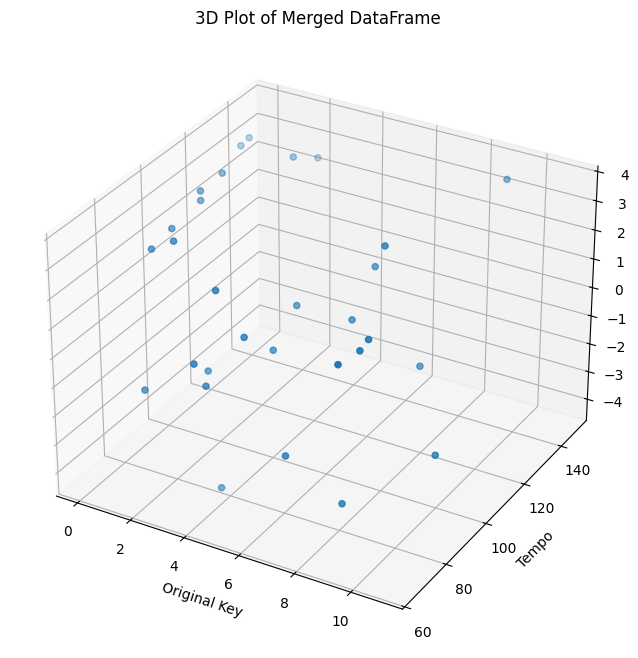
\includegraphics{./static/3d-plot.png}
\caption{The 3D plot of our dataset. The 3 dimensions are the song's
key, its tempo and the mean MFCC extracted from it.}\label{fig:3d-plot}
\end{figure}

Another approach that was tested was the usage of Spotify's Voyager
library \autocite{SpotifyVoyager2024} for the creation of the similarity
space and the \(K\)-NN graph. This approach was limited in regards to
the retrieval of the most dissimilar tracks and thus was discarded. Also
the K-Means algorithm was shortly examined as an alternative, but it
presented the same issue.

\section{Conclusion}\label{conclusion}

In this report, we presented our music recommendation system
implementation, that focuses on melodic, rhythmic and spectral features
for each similarity comparisons. Our results vary between the genres, in
large part due to common characteristics. For example, metal tracks are
most distinguishable from the others, due to their fast beat and
spectral maximalism. In contrast, some jazz songs where found to be
similar with some rock ones. At first glance this would seem to be a
flaw of our system, but by listening to the query song and the
recommendations we came to the conclusion that they \emph{do} actually
share a lot of elements and can be thought of as neighbors in our small
dataset.

\section{Task separation}\label{task-separation}

\begin{itemize}
\tightlist
\item
  Harmony and Melody feature exploration was done by Konstantinos
  Chousos.
\item
  Rhythm and Tempo feature exploration was done by Vasileios Katsaitis.
\item
  Timbre and Spectral Shape feature exploration was done by Dimokritos
  Kolitsos.
\end{itemize}

\printbibliography

\end{document}
